%!TEX root = TQFTbook.tex
%%%%%%%%%%%%%%%%%%%%%%%%%%%%%%
\chapter{Turaev--Viro theory}\label{c:TV}



In this chapter, we define an extended 3-dimensional TQFT called
Turaev--Viro theory. It will be defined as a lattice theory: we will define
$Z(M)$ by choosing a cell decomposition of $M$, writing $Z(M)$ as a state
sum, and then proving that it is independent of the choice of cell
decomposition. In many ways, it is very similar to the definition of
2-dimensional FHK theory in \chref{c:2d-lattice}, but replacing a separable
symmetric Frobenius algebra by a spherical fusion category $\calC$.

This theory was introduced by Turaev and Viro \cite{turaev-viro} in the
special case  when $\calC$ is the category of representations of quantum
group $U_q\su(2)$ with $q$ being a root of unity; in their work, they only
considered the usual (unextended) theory. It was generalized in
\cite{barrett} to arbitrary spherical fusion categories (again, as an
unextended theory); in fact, this was the motivation for introducing the
notion of a spherical fusion category. Extension to 3-2-1 theory was done 
in the series of papers \cite{balsam-kirillov}, 
\cite{balsam-TV2}, \cite{balsam-TV3}. 
Extension down to a point is fairly obvious (we were just too lazy to write 
it down).

Throughout this chapter, $\calC$ is a spherical fusion category over an
algebraically closed field $\kk$ of characteristic zero. We keep all
notation from the previous chapter, in particular denoting by $\OC$ the set
of isomorphism classes of simple objects in $\calC$ and choosing a
representative $X_i$ for each $i\in \OC$. We denote by $E$ the set of oriented
 edges (1-cells) of $M$. A manifold with a choice of PLCW decomposition will be 
 called a combinatorial manifold. Our main reference is \cite{balsam-kirillov}.



%%%%%%%%%%
\section{Turaev--Viro theory in dimensions $0,1$}\label{s:tv-dim01}

Similar to the case of extended 2d TQFT, here we define

$$
Z_\calC(\bullet^+)=\calC, \qquad
Z_\calC(\bullet^-)=\calC^\op
$$

Since the empty zero-dimensional manifold $\emptyset_0$ is the unit under disjoint union,
it must be assigned the unit under Deligne tensor product:

$$
Z_\calC( \emptyset_0)=\vecf
$$

To each unoriented edge $r \in E$, assign an object
\[
E_r = \bigoplus_{i \in \OC}  X_i \boxtimes X_i^* \in \calC_{r'} \boxtimes \calC_{r''}
\]
where $r',r''$ are two possible orientations of $r$. Because of symmetry of $E_r$ ( see \leref{l:spherical-E} ),
 it doesn't matter which orientation is labelled $r'$ or $r''$.

For an oriented 1-manifold $N$ ( possibly with a boundary ) we choose a cell decompostion of it and define
\[
Z_\calC (N) = \dots \boxtimes_\calC \calC \boxtimes_\calC \calC \dots
\]
where a $\calC$ comes from each edge, and a $\boxtimes_\calC$ comes from each internal vertex. ( This is analogous to 
\eqref{e:ZAN-def}, with quotient being achieved by the balanced tensor product. See figure below for a visualization. )

\begin{center}
   	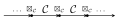
\includegraphics{figures/c19-fig01.svg}
\end{center}

As can be easily shown using \leref{l:bimodule-composition}, this assigns the bimodule category 
$_\calC \calC_\calC$ to an interval ( independent of the cell decomposition )

$$
Z_\calC(I) =  \calC \boxtimes_\calC \boxtimes_\calC \cdots \calC \simeq \calC
$$


This matches with our expectation. Since, the ordinary interval is the identity cobordism of the 
positively oriented point, it should be assigned the identity 1-morphism of $\calC$, which is 
the bimodule category $_\calC \calC_\calC$.

\begin{exercise}
	Show that $Z_\calC ( S^1 ) \simeq \calZ(\calC)$. ( Recall from \thref{t:cat-trace} and \thref{t:category-inv-coinv} 
	that $ \circtensor \calC \simeq  \calC\boxtimes_{\calC^e} \calC \simeq  \calZ(\calC) $. )
\end{exercise}

Since the one-dimensional empty manifold $\emptyset_1$ is unit under disjoint union of one-manifolds, it should 
be assigned $\vecf$ ( as bimodule over $\vecf$ ) by $Z$ functor:

\[
Z_{\calC}(\emptyset_1)=\vecf
\]

We used the subscript $\calC$ in this section just to emphasize that the assignment of data by a Turaev--Viro TQFT 
depends on the choice of $\calC$. We will suppress this subscript in the remaining sections.
%%%%%%%%%%
\section{Turaev--Viro theory in dimension $2$}\label{s:tv-dim2}

We will now consider what kind of data is assigned by $Z$ to a two-dimensional surface $N$. When
 $\partial N = \emptyset$, $Z(N)$ should be a functor from $Z(\emptyset_1)$ to $Z(\emptyset_1)$.

\[ 
Z(N): \vecf \rightarrow \vecf
\]

\begin{exercise}
	Show that $Z(N): \vecf \rightarrow \vecf$ is naturally isomorphic to tensoring with the vector space 
	$$ W_N := Z(N)(\kk).$$ Namely for any vector space $V \in \vecf$, we have $Z(N)(V) \simeq W_M \otimes_\kk V$. 
	Thus we may identify the functor $Z(N)$ with the vector space space $W_N$.
\end{exercise}

This exercise agrees with our expectation that a 3d TQFT should assign a vector space to a closed two-dimensional surface.


More generally, if $\partial N \ne \emptyset$, $Z(N)$ is a functor from the finite abelian category $Z(\ov{\partial  N})$ 
to $\vecf$. Here again we are considering $N$ as a bordism from $\partial N$ to the empty set ( similar to \chref{c:2d-lattice} ).

\[
Z(N): Z(\ov{\partial  N}) \rightarrow \vecf
\]


For a 2-cell $C$ with $n$ edges along it's boundary, this should be a functor:
\[
Z(C):\calC^{\boxtimes n}\to \vecf
\]


Following the general recipe of lattice/state-sum models, 
we will ( soon ) define an invariant of a 3d manifold $M$ by labelling the edges in its cell decomposition by objects of $\calC$.
The orientation and edge labels for 2-cells will be induced from that 3d data. For that purpose, it will be useful to have the 
following defintion.

\begin{definition}
	A labeling of $M$ is a map $l:E \rightarrow \OC $ which assigns to every oriented edge $e$ of $M$ an object $l(e) \in \OC$ 
	such that $l(\ov{e})=l(e)^*$. A labeling is called simple if for every edge, $l(e)$ is simple.
	
	Two labeling $l_1$ and $l_2$ are called equivalent if $l_1(e) \simeq l_2(e)$ for every $e \in E$.

\end{definition}


%%%%%%%%%%%%%%   
\begin{figure}[ht]
	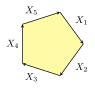
\includegraphics{figures/c19-fig02.svg}
	\hspace{1.5cm} $H(C,l)=\<X_1,X_2,\dots, X_5\>$
	\caption{Defining the state space for a 2-cell}\label{f:state_space1}
\end{figure}
%%%%%%%%%%%%%%   

For a given labeling $l$, we define, for every oriented 2-cell $C$, the state space

\begin{equation}
	H(C,l)=\<l(e_1), l(e_2),\dots, l(e_n)\>,\qquad 
	\del C=e_1\cup e_2\dots\cup e_n
\end{equation}

where the edges $e_1,\dots, e_n$ are taken in the clockwise order on
$\del C$ as shown in \firef{f:state_space1}. The functor $\<\dots\>$ was defined and studied in \seref{s:cat-pairing}. 
In particular, the space $\<c_1,c_2,\dots,c_n\>$ only depends on the cyclic order $c_1,c_2,\cdots,c_n$, and 
not on the starting edge.

For an oriented 2-dimensional combinatorial manifold $N$, we define

\begin{equation}
	H(N, l)= \bigotimes_{C} H(C, l)
\end{equation}

where the product is over all 2-cells. Orientation on each 2-cell $C$ is induced from the orientation of $N$.

\begin{equation}
	H(N,l)=\bigoplus_l H(N,l)
\end{equation}

Finally, we define the state space assigned by the Turaev--Viro theory to $N$ as

\begin{equation}\label{d:TV-surface}
	H(N)= \bigoplus_l H(N,l)
\end{equation}

where the sum is over all simple labelings up to equivalence.

Note that it follows from \eqref{e:dual} that we have canonical isomorphism
\begin{equation}\label{e:H-duality}
	H(\ov{N}) = H(N)^*
\end{equation}

 We have used the notation $H(N)$ for the $Z(N)$ functor in this section to suggest that this data corresponds to 
 the state space associated with the surface $N$. This notation also helps distinguish this assignment from the additional 
 3d-data introduced in the next section.

%%%%%%%%%%
\section{Turaev--Viro theory: full definition}\label{s:tv-full-definition}
We now define the TV invariant of 3-manifolds. Let $M$ be a combinatorial 3-manifold with boundary. We fix a labeling $l$
 of edges of $M$. Then we can assign a vector $Z(F,l) \in H(\partial F, l)$ to  every 3-cell $F$ as follows. Recall that $F$ is an
  inclusion $F:(0,1)^3 \rightarrow M$. The pullback of PLCW decomposition of $M$ gives a PLCW decomposition of 
  $\partial (0,1)^3 \simeq S^2$. Consider the dual graph $\Gamma$ of this decomposition and choose an orientation for every 
  edge of this dual graph ( arbitrarily ) as shown in \firef{f:dual_graph}.

%%%%%%%%%%%%%%
\begin{figure}[ht]
	\centering
	
	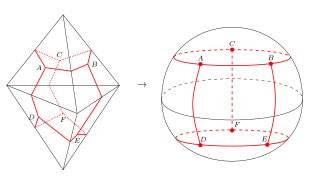
\includegraphics{figures/c19-fig03.svg}
	\caption{The dual graph on the boundary of a 3-cell}\label{f:dual_graph}
\end{figure}
%%%%%%%%%%%%%%

Note that a labeling $l$ of $M$ defines a labeling of edges of this dual graph as shown in figure \firef{f:state_space2}. 
Moreover, choose, for every face $C \in \partial F$, an element $\ph_C \in H(C,l)^*=\<l(e_n)^*,\dots,l(e_1)\>$. Then this 
collection of mrohisms defines a coloring of vertices of $\Gamma$.

By \leref{l:colored-spherical}, we get an invariant $\<\Ga\>_{S^2\setminus\{p\}} \in \kk$, which depends on the choice of
 labeling of edges $l$ and on the choice of morphisms $\ph_C$. We define $Z(F,l) \in \otimes_C H(C,l)$ by

\begin{equation}
	(Z(F,l),\otimes \ph_C)=\<\Ga,l,\{ \ph_C\}\>_{S^2\setminus\{p\}}
\end{equation}

If $F$ is a tetrahedron, then this coincides with the definition in \cite{barrett}; if $\calC$ is the category of representations 
of quantum $\sll_2$, these numbers are the $6j$-symbols.

%%%%%%%%%%%%%%
\begin{figure}[ht]
	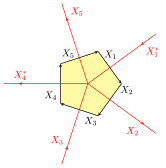
\includegraphics{figures/c19-fig04.svg}\qquad
	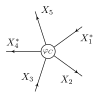
\includegraphics{figures/c19-fig05.svg}
	\qquad $\ph_C \in H(C,l)^*=\<X_5^*,X_4^*, \dots, X_1^*\>$
	\caption{Coloring of the dual graph}\label{f:state_space2}
\end{figure}
%%%%%%%%%%%%%%


We can now give a definition of the TV invariants of combinatorial 3-manifolds.

\begin{definition}\label{d:TV_invariant}
	Let $M$ be a combinatorial 3-manifold with boundary and $\calC$ - a spherical category. Then for any coloring $l$, 
	define a vector
	\[
		Z(M,l) \in H( \partial M,l)
	\]
	by
	\[
	Z(M,l) = \ev\left( \bigotimes_F Z(F,l) \right)
	\]
	where
	\begin{itemize}
		\item $F$ runs over all 3-cells in $M$, each taken with the induced orientation, so that 
		\[
		\bigotimes_F Z(F,l) \in \bigotimes_F H(\partial F,l) = H(\partial M,l) \otimes \bigotimes_c H(c',l) \otimes H(c'',l)
		\]
		\item $c$ runs over all unoriented 2-cells in the interior of $M$; $c'$,$c''$ are the two orientations of such a cell, so 
		that $c'=\ov{c''}$.
		\item $\ev$ is the tensor product over all $c$ of evaluation maps 
		$H(c',l)\otimes H(c'',l)=H(c',l)\otimes H(c',l)^* \rightarrow \kk$
	\end{itemize}
	Finally we define
	\[
	Z(M)= \DD^{-v (M)} \sum_{l} \left(  Z( M,l) \prod_{e} d^{n_e}_{l(e)} \right)
	\]
	where
	\begin{itemize}
		\item the sum is taken over all equivalence classes of simple labelings of $M$,
		\item $e$ runs over the set of all ( unoriented ) edges of $M$,
		\item $\DD$ is the dimension of the category ( defined in \thref{t:drinfeld-dim}), and $v(M)=$number 
		of internal vertices of $M$ + $\frac{1}{2}$(number of vertices on $\partial M$),
		\item $d_{l(e)} $ is the categorical dimension of $l(e)$, and
		$$ n_e = \begin{cases}
			1,\quad e \text{ is an internal edge}\\
			\tfrac{1}{2},\quad e\in \partial M
		\end{cases}
		$$
	\end{itemize}
\end{definition}

In the special case of a triangulated manifold, this coincides with the construction in \cite{barrett}.

\begin{theorem}\label{t:main1}
	If $M$ is a PL manifold without boundary, then the number $Z(M) \in \kk$ defined in \deref{d:TV_invariant} 
	does not depend on the choice of PLCW decomposition of $M$: for any two choices of PLCW decomposition, 
	the resulting invariants are equal.
\end{theorem}

The proofs for this theorem can be found in \cite{balsam-kirillov}.

Moreover, these invariants can be extended to a TQFT. Namely, let $M$ be a combinatorial 3-cobordism between 
two 2-dimensional combinatorial manifolds $N_1$,$N_2$, i.e. a combinatorial manifold $M$ with boundary such
 that $\partial M = \ov{N_1} \sqcup N_2$ ( note that the combinatorial structure on $M$ automatically defines a 
 combinatorial strucutre on $\partial M$). Then $H(\partial M)=H(N_1)^* \otimes H(N_2)=\mathrm{Hom}_\kk ( H(N_1),H(N_2))$, 
 so \deref{d:TV_invariant} defines a linear operator
\[
Z(M): H(N_1) \rightarrow H(N_2)
\]

\begin{theorem}\label{t:main2}
\par\noindent
	\begin{enumerate}
		\item So defined invariant satisfies gluing axiom: if $M$ is a combinatorial 3-manifold with boundary 
		$\partial M=N_0 \cup N \cup \ov{N}$, and $M'$ is the manifold obtained by identifying boundary components 
		$N$,$\ov{N}$ of $\partial M$ with the obvious cell decomposition, then we have
		\[
		Z(M')= \ev_{H(N)} Z(M) = \sum_a (Z(M),\ph_\alpha \otimes \ph^\alpha),
		\]
		where $\ev$ is the evaluation map $H(N)\otimes H(\ov{N}) \rightarrow  \kk $, and $\ph_\alpha \in H(N)$,
		 $\ph^\alpha \in H(\ov{N})$ are dual bases.
		\item If $M$ is a 3-manifold with boundary, and $M'$,$M''$ are two PLCW decompositions of $M$ which 
		agree on the boundary, then $Z(M')=Z(M'') \in H( \partial M')=H(\partial M'')$.
		\item For a combinatorial 2-manifold $N$, define $A_N:H(N) \rightarrow H(N)$ by
		\begin{equation}\label{e:projector}
			A_N=Z(N \times I)
		\end{equation}
		Then $A_N$ is a projector: $A^2_N = A_N$.
		\item For a combinatorial 2-manifold $N$, define the vector space
		\begin{equation}
			Z(N)= \mathrm{Im}(A_N:H(N) \rightarrow H(N))
		\end{equation}
		where $A$ is the projector \eqref{e:projector}. Then the space $\<N\>_{S^2\setminus\{p\}}$ is an invariant of PL 
		manifolds: if $N'$, $N''$ are two different PLCW decompositions of the same PL manifold N, then one has a
		 canonical isomorphism $Z(N') \simeq Z(N'')$.
		\item The assignments $N \mapsto Z(N), M \mapsto Z(M)$ give a functor from the category of PL 3-cobordisms
		 to the category of finite-dimensional vector spaces and thus define a 2+1 dimensional TQFT.
		\end{enumerate}
\end{theorem}

The proof to this theorem can also be found in \cite{balsam-kirillov}.

TODO: The following paragraph should be verified by AK.


 Balsam and Kirillov's state-sum construction  3-2-1 extends the Turaev-Viro 
 theory.  It's natural to ask if they could have fully extended it to a 3-2-1-0 TQFT.  
 In principle, this is doable. But this requires the full complexity of a weak 3 category.
In particular, all the equivalences between ( compositions of ) 1-morphisms 
should hold upto 2-morphisms, and ( compositions of ) 2-morphisms should hold 
 upto 3-morphisms. This leads to a very complicated web of coherence relations. 
 The extension to 0 dimensional manifolds requires a more workable definition of 
 an ($\infty$,3) category.


%%%%%%%%%%
\section{Proof of independence of PLCW decomposition}\label{s:proof}

In this section, we give proofs of \thref{t:main1}, \thref{t:main2},
i.e. prove that TV invariants are independent of the choice of PLCW
decomposition. Before giving the proof, we will enumerate the 
moves that were mentioned in \thref{t:plcw-moves}, in a form more suited 
to this chapter.

\begin{description}
	\item[M1: removing a vertex]
	Let $v$ be a vertex which has a neighborhood whose intersection with 
	the 2-skeleton is homeomorphic to the ``open book'' shown below with
	$k\ge 1$     leaves;    moreover, assume that all leaves in the
	figure are distinct 2-cells and the two
	1-cells  are also  distinct (i.e., not two ends of the same
	edge). Then move M1 removes vertex $v$ and replaces two 1-cells
	adjacent to it with a single 1-cell.
%%%%%%%%%%%%%%   
\begin{figure}[ht]
	\begin{center}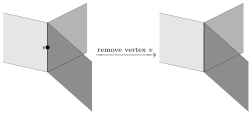
\includegraphics{figures/c19-eqfig02.svg}\end{center}
	\caption{Move M1}\label{f:movef1}
\end{figure}
%%%%%%%%%%%%%%   
	
	\item[M2: removing an edge]
	Let $e$ be a 1-cell which is regular and which is 
	adjacent to exactly two distinct 2-cells $c_1, c_2$ as shown in the
	figure below.  Then the move M2 removes the edge $e$ and replaces
	the cells $c_1,c_2$ with a  single cell $c$. 
%%%%%%%%%%%%%%   
\begin{figure}[ht]
	\begin{center}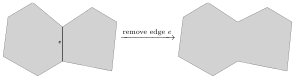
\includegraphics{figures/c19-eqfig03.svg}\end{center}
	\caption{Move M2}\label{f:movef2}
\end{figure}
%%%%%%%%%%%%%%   
	
	\item[M3: removing a 2-cell]
	Let $c$ be a 2-cell which is regular  and which is 
	adjacent to exactly two distinct 3-cells $F_1, F_2$ as shown in the
	figure below.  Then the move M2 removes the 2-cell $c$ and replaces the
	cells $F_1,F_2$ with a single cell $F$.
%%%%%%%%%%%%%%   
\begin{figure}[ht]
	\begin{center}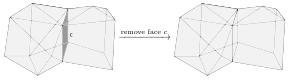
\includegraphics{figures/c19-eqfig04.svg}\end{center}
	\caption{Move M3}\label{f:movef3}
\end{figure}
%%%%%%%%%%%%%%   
	
\end{description}



We will now show that the TV state sum is invariant under M1--M3.

\subsection*{Invariance under M1}
First we consider move M1. Note that by applying M2 and M3, we can
transform an open book  with any number of pages to one with only one page
(see \firef{f:book}). 
\begin{figure}[ht]
	\begin{center}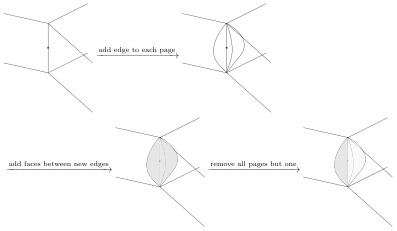
\includegraphics{figures/c19-eqfig05.svg}\end{center}
	\caption{Decomposing an open book into a single page book}\label{f:book}
\end{figure} 


Thus, it suffices to prove invariance under M1 in this
special case. Drawing the dual graph in the vicinity of the vertex,
invariance under M1 is equivalent to the following equality:
\begin{center}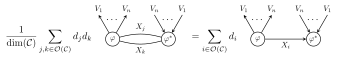
\includegraphics{figures/c19-eqfig06.svg}\end{center}
Note the normalizing factor
$\frac{1}{\mathcal{D}^2}$ which comes from the fact that we are removing a
vertex.

Using semisimplicity of $\C$, it is easy to see that it suffices to show
this equality in the special case when $V=V_1\otimes \dots \otimes V_n$ is
simple:
\begin{center}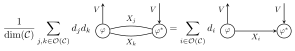
\includegraphics{figures/c19-eqfig07.svg}\end{center}

By \leref{l:pairing}, the right-hand side is equal to $\coev_V\colon \one
\to V\otimes V^*$. Since $\Hom(\one, V\otimes V^*)$ is one-dimensional,
the left-hand side is also a multiple of $\coev_V$. Composing it with the
evaluation morphism  $\ev_V$, we get
\begin{align*}
	&\frac{1}{\DD}\sum_{j,k}d_jd_kN_{1}^{Vjk} =
	\frac{1}{\DD}\sum_{j,k}N_{k^*}^{Vj}d_kd_j\\
	&\quad=\frac{1}{\DD}\sum_{j}\Bigl(\sum_{k}N_{k^*}^{Vj}d_k\Bigr)d_j=
	\frac{1}{\DD}\sum_{j}(d_{V}d_j)d_j=d_V,
\end{align*}
which proves that the left-hand side is equal to $\coev_V$.






\subsection*{Invariance under M2}
The invariance under M2 is seen as follows. By definition, the edge being
removed is incident to exactly two faces $c_1, c_2$. Each face bounds the
same two 3-cells $F_1, F_2$. In  \firef{f:move2}, we draw the dual graphs.
In each of the summands we have two graphs corresponding to cells $F_1,
F_2$, separated by a dot.  The equality follows
immediately from the fact that if $\ph_\al,\ph^\al$ and $\psi_\be,\psi^\be$ 
are dual bases, then so are $\ph_\al\ccc{X_i}\psi_\be$, $\psi^\be\ccc{X_i^*}\ph^\al$ 
(cf. \coref{c:composition2}). 
\begin{figure}[ht]
	\begin{center}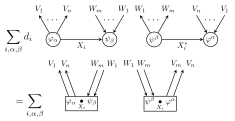
\includegraphics{figures/c19-eqfig08.svg}\end{center}
	\caption{}\label{f:move2}
\end{figure}

\subsection*{Invariance under M3}
Finally, we consider M3. In this case the invaraince immediately follows
from \leref{l:pairing2}, whith  two subgraphs corresponding to two 3-cells
separated by the 2-cell being removed.


%%%%%%%%%%%%%%%%%%%%%%%%%%%%%%%%
\section{String-net model}\label{s:stringnet}


In this section we look at a physics model which, in a certain limit, is described 
by Turaev--Viro TQFT. This model was introduced  by Levin-Wen \cite{levin-wen}, 
and is known as the string-net model. Roughly speaking, a state in this model
consists of highly fluctuating ``string-nets'' on a closed surface $N$, which are  
colored graphs on $N$ modulo some local relations. The allowed graphs
on these string-nets alongwith the local relations encode the data of a spherical
fusion category $\calC$.  We will here outline the correspondence between the string-net
 model and Turaev--Viro TQFT. Formal details, including the most
general proof for this correspondence can be found in \cite{kirillov-stringnet}. 
We also use this section to make some general comments about how TQFTs are viewed
in relation to gapped quantum systems in physics.


Using the \deref{d:colored-graph} of a colored graph, we denote
  $$
\mathrm{Graph}(N)=\text{set of all $\calC$-colored graphs in $N$ }
$$

We can also consider formal linear combinations of colored graphs. 
We denote
 $$
\mathrm{VGraph}(N)=\text{formal linear combinations of graphs }\Gamma \in \mathrm{Graph}(N) 
$$

\begin{definition}\label{d:null-graph}
	Let $D \in N$ be an embedded disk. We define a null graph $\boldsymbol{\Gamma} = c_1 \Gamma_1 + \cdots + c_n \Gamma_n 
	\in \mathrm{VGraph}(N)$ to be a linear combination of clolored graphs in $N$ such that:
	\begin{enumerate}
		\item $\Gamma$ is transerversal to $\del D$ (i.e., no vertices of $\Gamma_i$ are on the boundary 
		of $D$ and edges of each $\Gamma_i$ meet $\del D$ transversally).
		\item  All $\Gamma_i$ coincide outside of $D$.
		\item $\< \boldsymbol{\Gamma} \>_D = \sum c_i \< \Gamma_i \cap D \>_D =0$, where 
		$ \< \Gamma_i \cap D \>_D$ is the expectation value defined by \thref{t:evaluation-disk}.
	\end{enumerate}
\end{definition}

The local relations ( adapted to our discussion ) are given in \firef{f:local_rels1}. More physics
oriented illustrations of local relations can be found in the original paper \cite{levin-wen}.

\begin{definition}
	Let $N$ be an oriented closed surface. The string-net space $H^{string}(N)$ is the quotient space
	\[
		H^{string}(N) = \mathrm{VGraph}(N)/\mathrm{VGraph}_0(N)
	\]
	where $\mathrm{VGraph}_0(N)$ is the subspace spanned by null graphs ( for all possible embedded 
	disks $D \in N$).
\end{definition}

The correspondence between Turaev--Viro TQFT and string-net models is the 
following theorem.

\begin{theorem}\label{t:tv-equals-stringnet}
	Let $N$ be a closed oriented surface. Then one has a canonical isomorphism
	\[
		H^{string}(N) \simeq Z(N),
	\]
	where the Turaev--Viro functor $Z(N)$ was defined in \deref{d:TV-surface}.
\end{theorem}

In fact, the correspondence can also be extended to surfaces with boundaries. 
In the languge of string-nets, surfaces with boundaries describe excited states. 
A surface with boundaries can be obtained from an oriented closed surface
by removing some discs. These would-be-discs are said to host quasiparticles 
or anyons. Different possible quasiparticles in the string-net model are given 
by the simple objects of $\calZ(\calC)$ --- the Drinfeld center of $\calC$. 
The proof and the precise statement can again be found in \cite{kirillov-stringnet}.
Heuristically, a quasiparticle must admit a consistent rule for moving any string labeled
by an object of $\calC$ past it. Such a rule is precisely the half-braiding, and its
compatibility with the tensor product of $\calC$ is the hexagon axiom 
(compare \deref{d:drinfeld-center}).

The string-net model provides a microscopic Hamiltonian ( on a lattice ) for the given
spherical fusion category $\calC$. The 
Hamiltonian operator is engineered such the its
ground states necessarily obey the local relations. The states invariant under
the local moves are constructed by taking superposition of all graphs
related through local moves. In this sense, the ground states in the string-net model are
described as fluctuating string-nets, or condensed string-nets. Note that the actual 
string-net model has excited states too, but their energy gap relative to the
ground state(s) is large enough that they can be ignored while working with low
energy processes. We say that the string-net model is ``gapped'', and the model
flows ( under renormalization ) to a TQFT.
This is a recurring theme in the physics literature: the low energy
limit of a gapped quantum system is described by a TQFT. After enough coarse-graining,
any observable should be insensitive to local relations. The microscopic details,
including the choice of lattice, get washed out when the theory reaches the low energy 
fixed point of the renormalization group flow. This was partly the motivation used by Levin-Wen 
to come up with the string-net model.



%%%%%%%%%%
\section{Example: Dijkgraaf--Witten in 3 dimensions}\label{s:tv-dw3}
In this section we look at an explicit example. We consider $\calC = \vect_G$, which was defined in \exref{x:vecg}. 
We choose $G$ to be some finite group, and the underlying field is $\C$ . We shall see that the Turaev--Viro theory 
associated to this $\calC$ is the Dijkgraaf--Witten theory in 3 dimensions. We refer the reader to 
\cite[Theorem 4.2]{petit} for a proof.

The simple objects in $\calC$ are complex one-dimensional spaces graded with an element $g \in G$. We 
denote such a simple object as $\C_g$. A simple labeling $l$ will assign a group element $g_e$ to every oriented edge.
To a $n$-side face whose boundary labels are ${g_1},\dots,{g_n}$ ( in cylic order ), the functor $Z$ assigns
\begin{align}\label{e:flatness}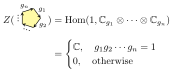
\includegraphics{figures/c19-eqfig01.svg}\end{align}

So the state space $H(N)$ for a 2-dimensional manifold $N$ is the space of flat $G$-connections. The categorical 
dimension of each edge is $1$ for $\calC$ . This gives $\mathrm{dim}(\calC)= |G|$. The projector $A_N$ thus 
takes the form
\[
A_N = \frac{1}{|G|^{v(N \times I)}}   \sum_{l_{\mathrm{flat}} } \left(  Z( N \times I ,l_{\mathrm{flat}}) \right).
\]

For a state $|a \> \in H(N)$, the sum over all flat gauge configurations $l_\mathrm{flat}$ on $N \times I$ gives a sum
 over all states $| h.a \>$, that are connected to $|a\>$ via some some element $h$ of the gauge group $G^{v(N)}$.
  As shown in \firef{f:flat-guage-configuration}, for each labeling $|a \>$ of $N$, an element $h \in G^{v(N)}$ leads 
  to another labeling $| b \>$ that is related to $| a \>$ by a gauge transformation. So the action of averaging 
  over $G^{v(N)}$ projects the states in $H(N)$ to $G^{v(N)}$-invariant states.  Thus $Z(N)$ is precisely the vector 
  space spanned by gauge equivalence classes of $G$-connections on $N$.


\begin{figure}[ht]
	\centering
	   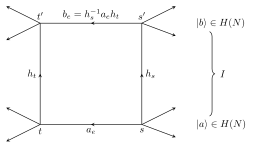
\includegraphics{figures/c19-fig06.svg}
\caption{A sample configuration appearing in the $\sum_{l_{\mathrm{flat}}} Z(N \times I , l_{\mathrm{flat}} )$. 
	Bottom of the diagram shows a portion of configuration $| a \>$ assigned to a closed 2-manifold $N$. $|a\>$ 
	assigns an $a_e \in G$ to each edge $e$, but we are showing only the edge $e$ between $s$ and $t$ here. 
	We label the vertical edges by elements $h_v$ of $G^{v(N)}$ for each $v \in v(N)$. 
	The flatness condition imposes that the configuration $|b\>$ on the other end of interval $I$ is a 
	gauge transformation of $|a\>$, i.e. $|b\>=|h.a\>$.}
\label{f:flat-guage-configuration}
\end{figure}

Similarly, for a 3-dimensional manifold $M$, we have
\begin{equation}\label{e:untwisted-DW}
	Z(M) = \frac{1}{|G|^{v(M)}} (\text{number of flat colorings})
\end{equation}
For a closed manifold, this counts isomorphism classes of principal G-bundles on $M$ ( with the appropriate
 weight that was described in \seref{s:DW-definition} ). This is same as the untwisted Dijkgraaf--Witten theory
  in 3 dimensions.


We can generalize this example by considering $\calC = \vect_G^\omega$ as was defined in \exref{x:vecg-twisted}. 
The choice of the 3-cocycle $\omega$ does not change the flatness condition coming from \eqref{e:flatness}. 
But the contribution $\<\Ga,l,\{ \ph_C\}\>_{S^2\setminus\{p\}}$ 
 coming from each oriented 3-cell $[0,1,2,3]$ now gets modified by $\omega(g_{01},g_{12},g_{23})$ or 
 $\omega(g_{01},g_{12},g_{23})^{-1}$ depending on its orientation with respect to the manifold $M$. Note that a 3-cell 
 has only 3 independent edge labels due to flatness condition. The Turaev--Viro partition function then takes the form
\begin{equation}\label{e:twisted-DW}
Z(M) = \frac{1}{|G|^{v(M)}} \sum_{l_\mathrm{flat}} \prod_{c \in \mathrm{3-cells}} \omega(g_1(c),g_2(c),g_3(c))^{\sigma(c)}
\end{equation}
where $\sigma(c) = \pm 1 $ depending on the relative orientation of the 3-cell $c$ with respect to $M$, and 
$g_1(c),g_2(c),g_3(c)$ are group elements labelling the edges of $c$ in a certain order. This turns out to be 
the state sum defintion of the twisted 3-dimensional Dijkgraaf--Witten theory ( compare \eqref{e:DW-integral} ). The
 untwisted theory \eqref{e:untwisted-DW} can be obtained from \eqref{e:twisted-DW} by settings $\omega=1$.


It is worth commenting here that Turaev--Viro TQFTs based on $\vect_G$, with $G$ a finite abelian group,
 are also very interesting from the physics perspective. These TQFTs describe the topological phases realized 
 by quantum double models. In particular, the simple objects in $Z(S^1)$ correspond to anyons in a 
 quantum double model, which have potential applications in topological quantum computing. A famous example
  is Kitaev's toric code \cite{kitaev}, which is based on $G=\Z_2$.


%%%%%%%%%%%%%%%%%%%%
\section{Comparison with cobordism hypothesis}\label{auto:c19-TV-comparison-with-cobordism-hypothesis}
FIXME: discuss relation of this to the construction fo extended 3d TQFT via cobordims hypothesis, see Chapter 17. 